\documentclass[a4paper, 12pt, oneside, titlepage]{article} %{\parskip}
\usepackage[top=2.54cm, bottom=2.54cm, left=3cm, right=2cm]{geometry}
\usepackage[utf8]{inputenc}
\usepackage[czech]{babel}
\usepackage[T1]{fontenc}
\usepackage{graphicx}
\usepackage{booktabs}
\usepackage{tabularx}
\usepackage{array}
\usepackage{indentfirst}
\usepackage{multicol}
\usepackage{titlesec}
\usepackage{mathtools}
\usepackage{esvect}

\usepackage{url}
\usepackage{caption}
\usepackage{subfig}
\usepackage[section]{placeins}
\usepackage{pdfpages}



\hyphenation{po-ly-gon}

\newcommand{\tg}{\mathop{\rm tg}\nolimits}
\newcommand{\arctg}{\mathop{\rm arctg}\nolimits}
\newtheorem{defin}{Definice}

\begin{document}

%\pagestyle{empty}
\setcounter{page}{1}   % nastaví čítač stránek znovu od jedné
\pagenumbering{arabic} % číslování arabskými
\thispagestyle{empty}

\begin{center}

\large

\v{C}eské vysoké učení technické v~Praze

\medskip

Fakulta stavební
\medskip

Katedra geomatiky

\vfill
\centerline{\mbox{
\includegraphics[scale=1.3]{obrazky/symbol_cvut_konturova_verze.jpg}} }


{\bf\Large Technická zpráva}

\vfill

{\bf\LARGE\bfseries Algoritmy v digitální kartografii}

\vfill

{\bf\Large Úloha č. 3: Digitální model terénu}


\vfill



\vfill
\vspace{5mm}

\begin{tabular}{c}

{\bf Bc. Pane Kuzmanov}\\
\noalign{\vspace{2mm}}
{\bf Bc. František Mužík}\\
\noalign{\vspace{10mm}}

Studijní program: Geodézie a kartografie \\
\noalign{\vspace{2mm}}

Specializace: Geomatika\\

\end{tabular}


\vfill

% Zde doplňte rok
Praha 2021

\end{center}

%---------------------------------------------------------------------
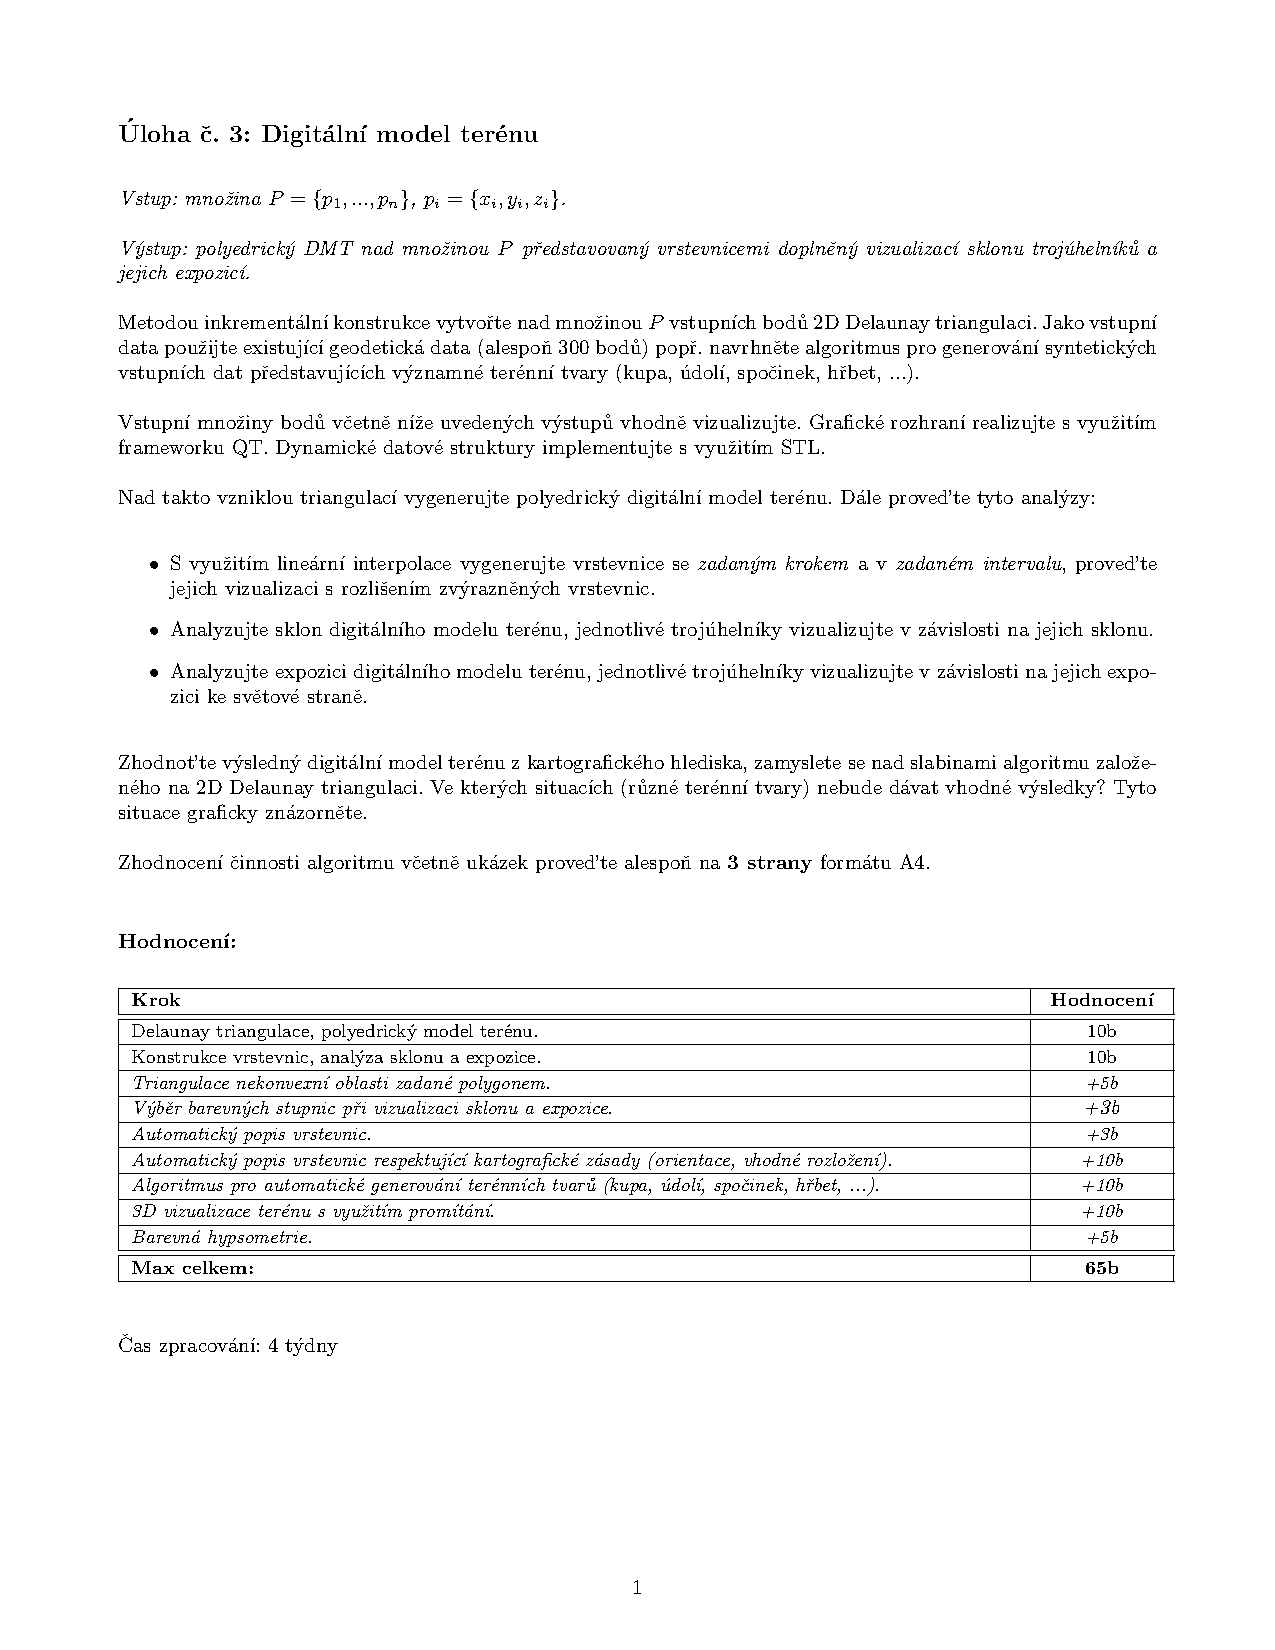
\includepdf{adkcv3}

%---------------------------------------------------------------------
\clearpage
\section{Údaje o bonusových úlohách}
\subsection{Triangulace nekonvexní oblasti zadané polygonem (+5b)}

\subsection{Výběr barevných stupnic při vizualizaci sklonu a expozice (+3b)}
Byla implementována možnost výběru dvou barevných palet pro každou z vizualizací. Pro sklon terénu je možné zvolit jednu z variant "Grayscale"~--~odstíny šedé nebo "Yellow to Red"~--~žluto~--~červená paleta. Ve výběru pro expozici lze najít dvě možnosti: KM~--~zvolená námi (obr.~\ref{fig:expozice_barvy}) nebo barevnou paletu, kterou používá ArcGIS (obr.~\ref{fig:esri_expozice}). Detailnější popis je v kapitolách \ref{vyp_sklon} a \ref{vyp_exp}.


\subsection{Automatický popis vrstevnic (+3b)}
Byl implementován automatický popis hlavních vrstevnic. Hlavní vrstevnice je každá pátá vrstevnice, která je zároveň výrazněji vykreslená. Více informací je v~kapitole~\ref{popis_vrs}.

\subsection{Automatický popis vrstevnic respektující kartografické zásady (+10b)}

\subsection{Algoritmus pro automatické generováních terénních tvarů (+10b)}

\subsection{3D vizualizace terénu s využitím promítání (+10b)}

\subsection{Barevná hypsometrie (+5b)}



\section{Popis a rozbor problému}
Je zadaná množina bodů s~prostorovými souřadnicemi X,Y,Z. Nad těmito body je vytvořen polyedrický digitální model terénu s~využitím Delaunayho triangulace. Součástí řešení je taktéž tvorba vrstevnic, včetně jejich popisu. Dále je možné zobrazit sklon terénu (tedy sklon jednotlivých trojúhelníků v triangulaci) a expozici ke světovým stranám (rozděleno na 8 stran).


\section{Popisy algoritmů formálním jazykem} \label{popisalg}

\subsection{Delaunay triangulace} \label{dt}
Jedná se o~nejčastěji využívanou metodu triangulace. Základní funkčnost metody spočívá v~rozdělení množiny bodů tzv. Thiessenovými polygony, jejichž vlastností je ohraničení každého z~bodů vstupní množiny tak, aby z~každého místa v~ohraničeném polygonu byl nejbližším bodem právě ten ohraničený (obr.~\ref{fig:th_pol}). Hrany polygonů tvoří osu spojnice dvou bodů.

 \begin{figure}[!htb]
	\centering
	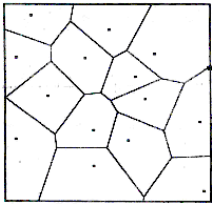
\includegraphics[scale=0.8]{obrazky/th_pol.png} 
	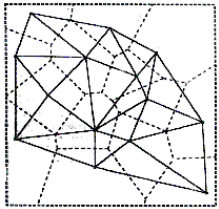
\includegraphics[scale=0.8]{obrazky/dt_obr.png}
	\caption{Ukázka Thiessenových polygonů (vlevo) a výsledné triangulace (vpravo) \cite{zcu}.
	}
	\label{fig:th_pol}
\end{figure} 
\FloatBarrier
 
Jestliže opsaná kružnice nad spojenou hranou dvou sousedních bodů neprotne jiný bod nebo jestliže se jiný bod nenachází uvnitř kružnice. Průběžným výpočtem je v~algoritmu vytvářen seznam hran (AEL~--~Active Edge List), pro které nebyl nalezen třetí bod pro triangulaci. Při nalezení nové hrany je potřeba zjistit, zda~--~se již nenachází v~AEL a tedy není případně duplicitní. Duplicitní hrany jsou odstraněny. Ve chvíli, kdy je AEL prázdný, je triangulace hotova. 

Nutné podmínky pro vytvoření triangulace:
\begin{itemize}
\item Žádný bod se nenachází uvnitř kružnice opsané libovolnému trojúhelníku triangulace.
\item Libovolné čtyři body by neměly ležet na kružnici~--~pak je triangulace nejednoznačná.
\item Maximalizace nejmenšího úhlu v trojúhelníku.
\item Splnění lokálních i globálních kritérií (vyvarování se tupých a velmi malých úhlů v~trojúhelníku, minimální suma délek stran...)
\end{itemize}

\textbf{Implementace algoritmu:} 
\begin{enumerate}
\item Nalezení náhodného a nejbližšího bodu: $p_1=rand(P), \Vert{p_1-p_2}\Vert=min.$
\item Vytvoř hranu $e=(p_1p_2)$
\item $\underline{p}=arg~min_{\forall p_i\in \sigma_L (e)}r^{'}(k_i),k_i=(a,b,p_i),e=(a,b)$
\item Pokud neexistuje $\underline{p}$, prohoď orientaci $e \leftarrow (p_2p_1)$. Jdi na 3)
\item Výpočet zbývajících hran trojúhelníka: $e_2=(p_2,\underline{p}),e_3=(\underline{p},p_1)$
\item Přidání 3 hran do AEL: $AEL \leftarrow e, AEL \leftarrow e_2, AEL \leftarrow e_3$
\item Přidání 3 hran do DT: $DT \leftarrow e, DT \leftarrow e_2, DT \leftarrow e_3$
\item Dokud AEL není prázdný:
\item \quad Vybrání první hrany z AEL: $AEL \rightarrow e, e=(p_1p_2)$
\item \quad Prohození její orientace: $e=(p_2p_1)$
\item \quad $\underline{p}=arg~min_{\forall p_i\in \sigma_L (e)}r^{'}(k_i),k_i=(a,b,p_i),e=(a,b)$
\item \quad Pokud existuje $\underline{p}$:
\item \quad \quad Zbývající hrany trojúhelníka: $e_2=(p_2,p),e_3=(\underline{p},p_1)$
\item \quad \quad Přidání hrany do DT, ale nikoliv do AEL: $DT \leftarrow e$
\item \quad \quad Přidání hrany do DT i do AEL: $add(e_2,AEL,DT), add(e_3,AEL,DT)$
\end{enumerate}

\subsection{Výpočet sklonu}\label{vyp_sklon}
Výpočet sklonu trojúhelníku je učen jako úhel~$\varphi$ mezi svislicí a normálou trojúhelníka~$n$. Výpočet probíhá vektorově nad každým z~trojúhelníků DMT. 

\begin{enumerate}
\item Určení vektorů $\overrightarrow{u}=(u_x,u_y,u_z)=(x_1-x_2, y_1-y_2, z_1-z_2), \overrightarrow{v}=(v_x,v_y,v_z)=(x_3-x_2,y_3-y_2,z_3-z_2)$ 
\item Výpočet normálového vektoru trojúhelníka: $\overrightarrow{n}=(n_y,n_y,n_z)=(u_y \cdot v_z-v_y \cdot u_z,-u_x \cdot v_z+v_x \cdot u_z,u_x \cdot v_y-v_x \cdot u_y)$
\item Sklon $\varphi =\dfrac{n_z}{\vert n\vert}$
\end{enumerate}

\subsubsection{Výběr barevné palety}
Trojúhelníky jsou vizualizovány na základě hodnoty~$\varphi$. Vizualizace je možná s~užitím dvou barevných palet. První možností jsou odstíny šedé

 \begin{figure}[!htb]
	\centering
	
\includegraphics[scale=0.11]{obrazky/gs.png} 
	
\includegraphics[scale=0.2]{obrazky/yr.png}
	\caption{Barevné palety pro vizualizaci sklonu terénu. Vlevo odstíny šedé a vpravo žluto~--~červená stupnice.
	}
	\label{fig:th_pol}
\end{figure} 
\FloatBarrier
\subsection{Výpočet expozice}\label{vyp_exp}
Výpočet expozice probíhá obdobným způsobem jako výpočet sklonu. V~podstatě jde o~úhel mezi x~--~ovou a y~--~ovou složkou normály trojúhelníka. Expozice určuje náklon trojúhelníka k jedné ze světových stran. V~aplikaci je uvažováno s~8 možnostmi (jih, jihozápad, západ, severozápad, sever, severovýchod, východ a  jihovýchod).

\begin{enumerate}
\item Určení vektorů $\overrightarrow{u}=(u_x,u_y,u_z)=(x_1-x_2, y_1-y_2, z_1-z_2), \overrightarrow{v}=(v_x,v_y,v_z)=(x_3-x_2,y_3-y_2,z_3-z_2)$ 
\item Výpočet normálového vektoru trojúhelníka: $\overrightarrow{n}=(n_y,n_y,n_z)=(u_y \cdot v_z-v_y \cdot u_z,-u_x \cdot v_z+v_x \cdot u_z,u_x \cdot v_y-v_x \cdot u_y)$
\item Určení expozice $exp=arccos\dfrac{n_z}{\vert n\vert}$
\end{enumerate}

\subsubsection{Výběr barevné palety}
Pro expozici jsou na výběr dvě možnosti barevných palet. Námi zvolená KM paleta a standardní paleta, kterou využívá např. ArcGIS.

\begin{figure}[!htb]
	\centering
	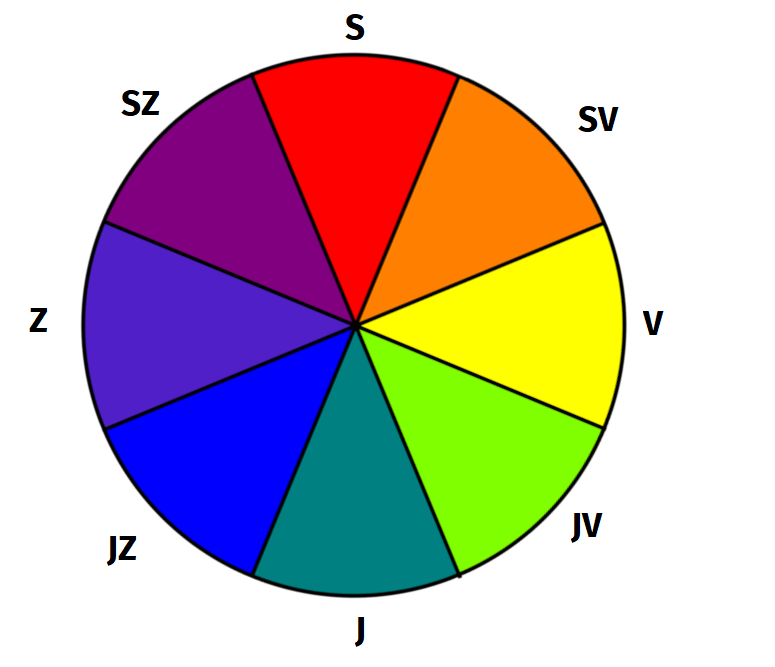
\includegraphics[scale=0.3]{obrazky/expozice_barvy.png} 
	\caption{KM barevná paleta pro vizualizaci expozice terénu.
	}
	\label{fig:expozice_barvy}
\end{figure} 
\FloatBarrier

\begin{figure}[!htb]
	\centering
	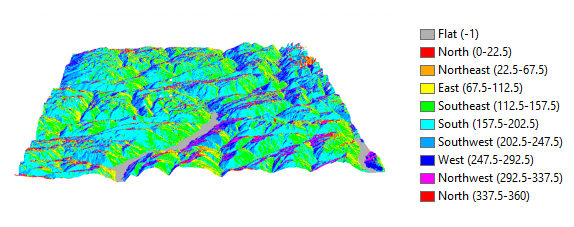
\includegraphics[scale=0.7]{obrazky/esri_expozice.png} 
	\caption{Vizualizace expozice terénu dle ArcGIS \cite{arcgispro}.
	}
	\label{fig:esri_expozice}
\end{figure} 
\FloatBarrier

\subsection{Výpočet vrstevnic}
Výpočet vrstevnic probíhá na základě vstupní Delaunayho triangulace, minimální a maximální výšky a rozestupu mezi vrstevnicemi. Jedná se o~určení vrstevnic lineární interpolací, předpoklad je tedy takový, že spád terénu je mezi podrobnými body konstantní. Jedná se o nejjednodušší a rozšířený způsob tvorby vrstevnic.

Nejprve je nutné zjistit, zda rovina $\rho$ protíná stranu $(p_i,p_{i+1})$ trojúhelníka:
\begin{enumerate}
\item Jestliže $(z-z_i)(z-z_{i+1})<0$, pak trojúhelník protíná rovinu~$\rho$ v~obecných bodech.
\item Jestliže $(z-z_i)(z-z_{i+1})>0$, pak trojúhelník neprotíná rovinu~$\rho$.
\item Jestliže $(z-z_i)(z-z_{i+1})=0$, pak jedna ze stran trojúhelníka leží v rovině~$\rho$.
\end{enumerate}

Výpočet souřadnic průsečíku A,B vrstevnice o~nadmořské výšce~$z$ s~trojúhelníkem tvořeným body 1,2,3:

\begin{center}
$x_A=\dfrac{x_3-x_1}{z_3-z_1}(z-z_1)+x_1$\\
$y_A=\dfrac{y_3-y_1}{z_3-z_1}(z-z_1)+y_1$\\
$x_B=\dfrac{x_2-x_1}{z_2-z_1}(z-z_1)+x_1$\\
$y_B=\dfrac{y_2-y_1}{z_2-z_1}(z-z_1)+y_1$\\
\end{center}

\subsubsection{Popis vrstevnice}\label{popis_vrs}
Automatický popis vrstevnic byl implementován pro každou hlavní vrstevnici (tedy každou pátou vrstevnici). Výškový údaj je vypsán nad vrstevnicí a umístěn v~polovině triangulačního trojúhelníka. 

Ve třídě Draw je implementace následovná:

\begin{verbatim}
      //Draw main contours label
       for (Edge mcl : main_contours_label)
       {
          //Start and end point of the contour edge
          QPoint3D sl_point = mcl.getStart();
          QPoint3D el_point = mcl.getEnd();

          //Get label coordintes
          QPoint3D label_point( (sl_point.x()+el_point.x())/2, 
                                (sl_point.y()+el_point.y())/2);

          //Draw Z coordinate
          QString z = QString::number(sl_point.getZ());
          qp.drawText(label_point, z);
       }
\end{verbatim}



\section{Problematické situace a jejich rozbor} \label{problemrozbor}
% (tj. simplexy) + ošetření těchto situací v kódu
\subsection{Automatické nastavení přechodné barevné stupnice mezi žlutou a červenou}
Pro zobrazení sklonu terénu byl zvolen přechod žluté do červené jako optimální varianta, nicméně vyladění správně plynule vykreslovaných barev bylo poměrně náročné k~představení. Naštěstí existují různé vizualizační online aplikace, které umí velice názorně pomoci~--~například \cite{rgbcol}.

\begin{verbatim}
void Draw::paintEvent(QPaintEvent *event)
{
...
        if (yelred == TRUE)
        {
        //Convert to color
        int col = 255 - k * slope;
        int colg = k * slope;
        QColor color(255, colg, col);

        //Set pen and brush
        qp.setBrush(color);
        qp.setPen(color);
        }
...
}
\end{verbatim}


\section{Vstupní data}
% formát vstupních dat, popis
Vstupem je textový soubor s~prostorovými souřadnicemi X,Y,Z geodetických bodů. Tyto body jsou považovány za vstupní množinu~P. Body byly získány exportem z~Digitálního modelu reliéfu 4.~generace \cite{ZABAGED} v prosředí ArcGIS~Pro \cite{arcgispro} (viz. obr. \ref{fig:arcgis_body}). 

\begin{figure}[!htb]
	\centering
	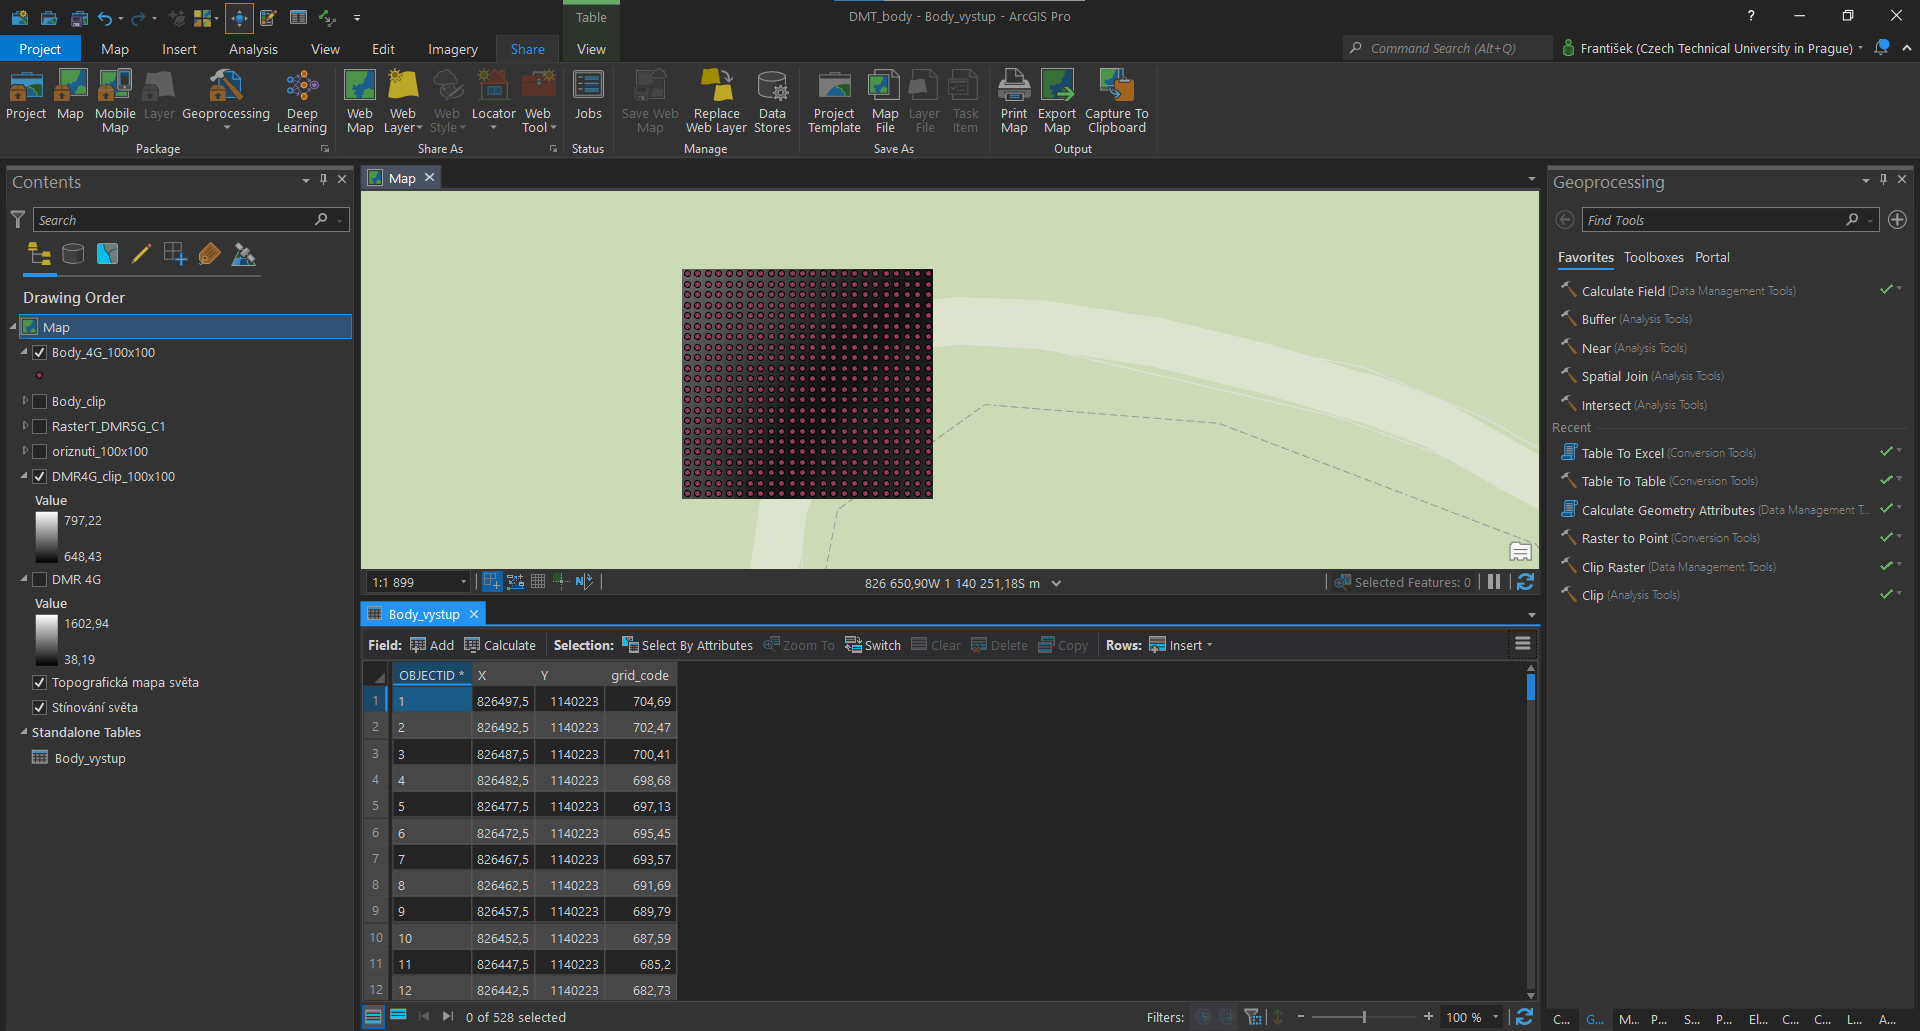
\includegraphics[scale=0.33]{obrazky/arcgis_body.png} 
	\caption{Export bodů v ArcGIS Pro z DMR4G na vybraném území.
	}
	\label{fig:arcgis_body}
\end{figure} 
\FloatBarrier

Formát vstupních dat je následující (ID, X, Y, Z):
\begin{verbatim}
1 846308.0 1129497.0 1141.2
2 846288.0 1129497.0 1131.8
3 846268.0 1129497.0 1123.2
...
\end{verbatim}


\section{Výstupní data}
% formát výstupních dat, popis
Za~výstup je považována grafický výstup vytvořené aplikace. Grafickým výstupem je polyedrický DMT nad množinou~P představovaný vrstevnicemi doplněný vizualizací sklonu trojúhelníků, jejich expozicí a vrstevnicemi s~popisem. 


\section{Snímky obrazovky vytvořené aplikace a její popis}



\section{Dokumentace}
% popis tříd, datových položek a jednotlivých metod
\subsection{Třída Algorithms}
Tato třída obsahuje výpočetní vzorce pro použité algoritmy.

\textbf{Třída algorithms obsahuje následující veřejné metody:}

\begin{verbatim}
double get2LinesAngle(QPoint &p1, QPoint &p2, QPoint &p3, QPoint &p4)
\end{verbatim}
Metoda vypočte velikost úhlu, který svírají dvě přímky. První přímku tvoří body $p_1, p_2$ a druhou přímku body $p_3, p_4$.\\

\begin{verbatim}
int getPointLinePosition(QPoint &a,QPoint &p1,QPoint &p2)
\end{verbatim}
Metoda určuje, zda~--~li bod leží v~levé či v~pravé polorovině od přímky (hrany polygonu). Vstupními parametry jsou určovaný bod~$a$ a body $p_1, p_2$, které tvoří přímku.\\

\begin{verbatim}
double getPointLineDistance(QPoint &a, QPoint &p1, QPoint &p2)
\end{verbatim}
Metoda určuje vzdálenost bodu~$a$ od přímky tvořenou body $p_1, p_2$.\\

\begin{verbatim}
QPolygon cHullJarvisScan(std::vector <QPoint> &points)
\end{verbatim}
Výpočet konvexní obálky načtených bodů na základě algoritmu Jarvis Scan (kapitola \ref{js}).\\

\begin{verbatim}
std::vector<QPoint> rotate(std::vector<QPoint> &points, double sigma)
\end{verbatim}
Otočení načtených bodů o~zadaný úhel $sigma$.\\

\begin{verbatim}
std::tuple<std::vector<QPoint>, double> minMaxBox(std::vector<QPoint> &points)
\end{verbatim}
Proměnná vracející min~--~max box, tedy vrcholy obdélníka a jeho výměru. Vstupem jsou načtené body.\\

\begin{verbatim}
QPolygon minAreaEnclosingRectangle(std::vector<QPoint> &points)
\end{verbatim}
Určení hlavního směru polygonu s využitím algoritmu Minimum Area Eclosing Rectangle (kapitola \ref{maer}). Na vstupu jsou body polygonu. Výstupem je generalizovaný a pootočený polygon.\\

\begin{verbatim}
QPolygon wallAverage(std::vector<QPoint> &points)
\end{verbatim}
Určení hlavního směru polygonu s využitím algoritmu Wall Average (kapitola \ref{wa}). Na vstupu jsou body polygonu. Výstupem je generalizovaný a pootočený polygon.\\

\begin{verbatim}
double LH(std::vector<QPoint> &points)
\end{verbatim}
Výpočet plochy obecného mnohoúhelníků pomocí LH vzorce.\\ 

\begin{verbatim}
std::vector<QPoint> resizeRectangle(std::vector<QPoint> &points, std::vector<QPoint> &er)
\end{verbatim}
Přepočet velikosti ohraničujícího obdélníku na základě výměry původního polygonu.\\

\begin{verbatim}
QPolygon longestEdge(std::vector<QPoint> &points)
\end{verbatim}
Určení hlavního směru polygonu s využitím algoritmu Longest Edge (kapitola \ref{le}). Na vstupu jsou body polygonu. Výstupem je generalizovaný a pootočený polygon.\\

\begin{verbatim}
QPolygon weightedBisector(std::vector<QPoint> &points)
\end{verbatim}
Určení hlavního směru polygonu s využitím algoritmu Weighted Bisector (kapitola \ref{wb}). Na vstupu jsou body polygonu. Výstupem je generalizovaný a pootočený polygon.\\

\begin{verbatim}
QPolygon cHullQuickHull(std::vector <QPoint> &points)
\end{verbatim}
Výpočet konvexní obálky načtených bodů na základě algoritmu Quick Hull (kapitola \ref{qh}).\\

\begin{verbatim}
void quickHullLocal(int ps, int pe, std::vector<QPoint> &points, QPolygon &ch)
\end{verbatim}
Metoda pro pomocný výpočet rekurentního určení konvexní obálky bodů algoritmem Quick Hull, lokální procedura (kapitola \ref{qh}). Vstupními parametry jsou indexy počátečního a koncového bodu $ps$ a $pe$ vstupní hrany, načtené body a konvexní obálka.\\

    
    
\subsection{Třída Draw}
Tato třída umožňuje vykreslování bodu a polygonů.

\textbf{Třída draw obsahuje následující privátní metody a proměnné:}
\begin{verbatim}
std::vector<QPoint> points
\end{verbatim}
Proměnná se souřadnicemi načtených bodů.\\

\begin{verbatim}
QPolygon ch, er;
\end{verbatim}
Polygony pro ukládání konvexní obálky a ohraničujícího obdélníku.\\

\begin{verbatim}
std::vector<QPolygon> polygons, chs, ers
\end{verbatim}
Proměnná uchovávající pomocné polygony v~průběhu výpočtu a pro vykreslení.\\


\textbf{Třída draw obsahuje následující veřejné metody a proměnné:}
\begin{verbatim}
explicit Draw(QWidget *parent = nullptr)
\end{verbatim}
Prvotní vykreslení bodu mimo okno aplikace.\\

\begin{verbatim}
void paintEvent(QPaintEvent *event)
\end{verbatim}
Metoda, která vykresluje bod či polygony.\\

\begin{verbatim}
void mousePressEvent(QMouseEvent *event)
\end{verbatim}
Metoda určující souřadnice určeného bodu.\\

\begin{verbatim}
void clearAddedData()
\end{verbatim}
Metoda mazající přidaná data z~obrazovky.\\

\begin{verbatim}
void clearDrawing()
\end{verbatim}
Metoda mazající nakreslený polygon z~obrazovky.\\

\begin{verbatim}
std::vector<QPoint> getPoints() {return points;}
\end{verbatim}
Vrací souřadnice lomových bodů polygonu.\\

\begin{verbatim}
std::vector<QPolygon> getPolygons(){return polygons;}
\end{verbatim}
Vrací souřadnice polygonů.\\

\begin{verbatim}
void setCh(QPolygon &ch_) {chs.push_back(ch_);}
\end{verbatim}
Nastavení polygonu konvexní obálky.\\

\begin{verbatim}
void setEr(QPolygon &er_) {ers.push_back(er_);}
\end{verbatim}
Nastavení polygonu ohraničujícího obdélníku.\\

\begin{verbatim}
void clearChs(){chs.clear();}
\end{verbatim}
Smazání polygonu konvexní obálky.\\

\begin{verbatim}
void clearErs(){ers.clear();}
\end{verbatim}
Smazání polygonu ohraničujícího obdélníku.\\

\begin{verbatim}
void drawPolygons(std::vector<QPolygon> &data);
\end{verbatim}
Vykreslení polygonů načtených z~textového souboru.\\

\subsection{Třída Load}
\textbf{Třída draw obsahuje následující veřejnou proměnnou:}
\begin{verbatim}
static std::vector<QPolygon> load_file(std::string &filename)
\end{verbatim}
Umožňuje načítání polygonů z textového souboru.\\

\subsection{Třída SortByX}
\textbf{Třída draw obsahuje následující veřejnou proměnnou:}
\begin{verbatim}
bool operator() (QPoint &p1, QPoint &p2)
\end{verbatim}
Ražení bodů dle jejich x~--~ové souřadnice.\\

\subsection{Třída SortByY}
\textbf{Třída draw obsahuje následující veřejnou proměnnou:}
\begin{verbatim}
bool operator() (QPoint &p1, QPoint &p2)
\end{verbatim}
Ražení bodů dle jejich y~--~ové souřadnice.\\

\subsection{Třída Widget}
Tato třída propojuje uživatelské rozhraní aplikace s kódem. Je vytvořena v sekci \emph{Design}.

\textbf{Třída widget obsahuje následující privátní metody a proměnné:}
\begin{verbatim}
void on_pushButtonClear_clicked()
\end{verbatim}
Vymazání kresby. Propojení s~tlačítkem \emph{Clear drawing}.\\

\begin{verbatim}
void on_pushButtonLoad_clicked()
\end{verbatim}
Načtení lomových bodů polygonů z~textového souboru. Propojení s~tlačítkem \emph{Load file with polygon}.\\

\begin{verbatim}
void on_pushButton_clicked()
\end{verbatim}
Spuštění funkce Building Simplify s~vybraným algoritmem. Propojení s~tlačítkem \emph{Building Simplify}.\\

\begin{verbatim}
void on_pushButtonClearData_clicked()
\end{verbatim}
Vymazání přidaných dat. Propojení s~tlačítkem \emph{Clear added data}.\\

\begin{verbatim}
void processPoints(std::vector<QPoint> &points)
\end{verbatim}
Volba použitého algoritmu na základě výběru z~combo boxů.\\



\section{Závěr}






\subsection{Možné či neřešené problémy} \label{mcn_problemy}


\subsection{Náměty na vylepšení} \label{vylepseni}



\begin{flushright}
V Praze 30.11.2021\\
\vspace{2mm}
Bc. Pane Kuzmanov\\
Bc. František Mužík\\
\end{flushright}


%---------------------------------------------------------------------
\clearpage 
\section*{Použitá literatura}
\renewcommand{\section}[2]{}%
\bibliographystyle{acm}
\bibliography{Literatura_u3_adk}


\end{document}
